\documentclass[12pt, letterpaper]{article}
\usepackage[utf8]{inputenc}
\usepackage[czech]{babel}
\usepackage[normalem]{ulem}
\usepackage{amsmath}
\usepackage{indentfirst}
\usepackage{listings}
\usepackage{caption}
\usepackage{float}
\usepackage{graphicx}
\usepackage{hyperref}
\usepackage{textcomp}
\usepackage{array}
%%%
%%%
\begin{document}
%%%
%%% TITLE PAGE
%%%
\begin{titlepage}
\centerline{
\includegraphics[width=10cm]{img/logo}}
\begin{center}
\vspace{30px}
{\huge
\textbf{Databázové systémy a metody zprac.inf.2}\\
\vspace{1cm}
}
{\Large
\textbf{KIV/DBM2}\\
\vspace{1cm}
}
{\large
\textbf{Porovnání úspěšnosti dle formy studia}\\
\textbf{Výtah}\\
\vspace{1cm}
}
\vspace{1cm}
{\large
Pavel Třeštík\\
}
{\normalsize
A23N0001P
}
\end{center}
\vspace{\fill}
\hfill
\begin{minipage}[t]{7cm}
\flushright
\today
\end{minipage}
\end{titlepage}
%%%
%%% TEXT START - Uvod
%%%
\section{Téma a motivace}
Vybraným tématem je \uv{porovnání úspěšnosti dle formy studia}. Hlavním cílem je zjistit úspěšnost každé formy studia
(prezenční, kombinované a distanční) a porovnat tyto úspěšnosti. Výsledkem tohoto porovnání by mělo být přibližně
stejné procento úspěšnosti.

Termín \uv{úspěšnost} byl již použit a nejjednodušší statistickou metrikou pro úspěšnost by byl jednoduše podíl
úspěšných absolventů ku všem studentům. Tato práce by ovšem neměla moc velký smysl, kdyby pro její dokončení stačilo 
udělat 3 podíly. Úspěšnost je zde pro nás tedy něco převážně neznámého a cílem práce je vybrat vhodné příznaky, které
nám úspěšnost vytvoří. Tato úspěšnost bude založena převážně na známkách. Známky jsou prakticky určeny k tomu, aby
ohodnocovaly studentovu úspěšnost. Čistě známka ovšem může být zkreslující údaj sám o sobě, protože předměty mohou
mít různé kreditové ohodnocení (tedy váhu), statut (A/B/C) a další. Také může hrát roli např. na kolikátý pokus
student známku dostal nebo jestli předmět opakuje.

Počítání úspěšnosti tímto způsobem by mohlo být možné analyticky či některým modelem strojového učení. V případě, že by
úspěšnost závisela na pouze malém počtu vlastností, jejichž důležitost je jasně daná, tak by bylo možné úspěšnost 
pouze vypočítat a výsledkem práce by mohl být pouze SQL skript. Při větším počtu vlastností nebo problémy s určením
jejich vah, bude nutné použít jiný přístup, kterým by nejspíše byl nějaký regresní algoritmus strojového učení. Důvodem
proč by se mohlo jednat o regresní úlohu je, že práce má vyjádřit úspěšnost pro danou formu studia. Otázkou ale je,
jak bude tato úspěšnost počítána.
%%%
%%% Realizace
%%%
\section{Realizace}
Prvním krokem k realizaci práce bylo vybrat vhodné data. Původní myšlenka byla vybrat co nejvíce sloupců a použitím 
nástroje \textbf{weka} postupně odebírat nepodstatné sloupce.

Výběr vhodných dat byl nakonec dělaný manuálně podle názvů sloupců a jejich popisků. Začalo se od tabulky 
\textbf{ZNAMKY}, protože ty jsou hlavním podkladem pro hodnocení úspěšnosti. Ke známkám se navíc přidaly některé
sloupce z jiných tabulek, které by mohly mít dopad na předpověď úspěšnosti např. \textbf{STUPEN\_PRED\_VZDELANI}.

Protože vymyslet způsob počítání úspěšnosti bez použití strojového učení je téměř nemožné, tak byl zvolen přístup
použití strojového učení. Vybírané sloupce proto byly voleny s ohledem na to, jak by se podle nich dal vytvořit model.

Pro vytvoření regresního modelu, který byl původní myšlenkou zadání by bylo potřeba mít nějaké reálné hodnoty, které 
úspěšnost určují. V datech takovýto údaj není, takže je potřeba údaj vytvořit a nebo změnit typ modelu.

Vzhledem k datům bylo rozhodnuto, že bude použit klasifikační model, protože s dostupnými daty lze poměrně snadno
vytvořit klasifikační třídy. Jako třídy byla použita boolean flaga, určující že student má záznam v tabulce 
\textbf{ABN\_ABSOLVENTI} a forma studia. Výsledkem je tedy 6 tříd z kombinace: 1 - absolvoval, 0 - neabsolvoval a 
P - prezenční, K - kombinovaný, D - distanční. Třída je tedy např. 1P, 0P, 1D,...

Vybraná data byla volena tak, aby se úspěšnost nevztahovala ke studentovi, ale spíše ke známkám. Následkem je, 
že za každého studenta může v datech být několik desítek záznamů. V době dokončení práce mají výsledná data 
\texttt{2722101} záznamů a z toho \texttt{461120} unikátních kombinací. Data povolují duplikáty, protože 
podle použitého modelu duplikáty mohou ovlivnit váhy modelu a tím model zpřesnit.

Kvůli datům bylo uděláno rozhodnutí, že model bude klasifikačním algoritmus. Jako hlavní model byl použit 
\textbf{Naivní Bayes}.
Bayes v této práci porušuje podmínku, že použité atributy by měly být nezávislé, ale i při porušení této podmínky je 
Bayes stále velmi dobrý klasifikátor. Důvod proč byl primárně použit Bayes je rychlost učení, kdy vytvoření modelu 
a cross-validace dat s 10ti iteracemi zabere přibližně 1 minutu.

Pro ověření modelu byl pokus použít i \textbf{SMO}, což by měla být implementace SVM. Problém s použitím tohoto modelu 
byl velice dlouhý čas učení modelu, kdy nad všemi daty nestačilo ani půl dne. Model je možné vytvořit během několika
minut, pokud je použit 50000 záznamů, což je pouze malý zlomek všech dat. Pro tento účel byl vyroben skript 
\texttt{50k\_data\_preparation.sql}. Bohužel ani s vytvořeným modelem se nepovedlo SMO použít, protože použit model
pro plný dataset je také úloha na minimálně několik desítek hodin. SMO byl proto opuštěn.
%%%
%%%
%%%
\section{Problémy}
Při výběru dat bylo poměrně těžké vhodně volit data bez znalosti databáze. Některé sloupce a jejich popisky nejsou 
zrovna nápomocné. Příkladem je zjištění absolventů, kteří jsou použiti k vyrobení tříd v datech. Tabulka 
\texttt{STUDENTI} má sloupec \texttt{Absolvent} s popiskem \uv{Absolvent}. Ze sloupce jde poznat, že se jedná o 
boolean hodnotu, ale už nejde poznat, jestli to značí úspěšného absolventa, studenta v posledním ročníku nebo co 
informace vlastně znamená. Jako indikace úspěšných absolventů byla použita existence záznamu v tabulce 
\texttt{ABN\_ABSOLVENTI}.

Také bylo poměrně těžké z dat vybrat nějaký vhodný způsob, který by sloužil k učení modelu. Původní myšlenka zadaní
byl regresní model, ale kvůli datum nešlo získat hodnoty pro učení regrese. Také se objevil nápad pouze shlukování,
či kombinace shlukování k postavení regresního modelu. Tento nápad byl zavrhnut, protože realizace by byla složitější
než se zdá. Protože už se nabízelo i shlukování, tak byl nakonec vybrán klasifikační model, pro který bylo možné 
vytvořit správná data a provést tak učení.

Problémem byl také dlouhý čas učení jiných modelů, než Naivní Bayes. Dle dostupných zdrojů je učení Bayese rychlejší
oproti jiným modelům, ale SMO model se nepovedlo natrénovat ani po zhruba 20ti hodinách, což je několika 1000 násobek
trénování Bayese. Resp. SMO se povedlo natrénovat v rámci minut na 50000 záznamech, což je zhruba 1.8\% datasetu.
Při zvýšení na 100000 záznamů už učení SMO trvalo několik hodin, po kterých bylo učení přerušeno.
%%%
%%% Vysledky
%%%
\section{Výsledky}
Práce měla porovnat úspěšnost dle formy studia. Důležité je zmínit, že výsledky nejsou poměr absolventů a studentů, 
ale poměr záznamů reprezentující známku a dodatečné informace k ní. Pro porovnání hlavních výsledků lze použít 
statistický podíl, proti výsledkům modelu.
\begin{table}[H]
    \begin{center}
        \begin{tabular}{ | c || c | c | }
            \hline
                        & Stat.     & N. Bayes    \\
            \hline \hline
            prezenční   & $\frac{335335}{2406529} = 13.93\%$    & $\frac{143168}{2406529} = 5.95\%$ \\
            \hline
            kombinované & $\frac{27727}{296209} = 9.36\%$       & $\frac{16371}{296209} = 5.53\%$   \\
            \hline
            distanční   & $\frac{2708}{19363} = 13.99\%$        & $\frac{1040}{19363} = 5.37\%$     \\
            \hline
        \end{tabular}
        \caption{Porovnání úspěšnosti modelu a statistiky}
        \label{table:main_result}
    \end{center}
\end{table}

Z tabulky \ref{table:main_result} vidíme, že výsledky modelu jsou značně horší, než reálné úspěšnosti. Důvodem nejspíš
je, že model velmi často zařazuje výsledky do opačné třídy. To naznačuje, že model je pravděpodobně nedostatečně 
obsáhlý proto, aby dokázal správně predikovat úspěšnost. Na obrázku \ref{fig:bayes_results} lze vidět výsledek klasifikace tímto modelem.
\begin{figure}[H]
    \centering
    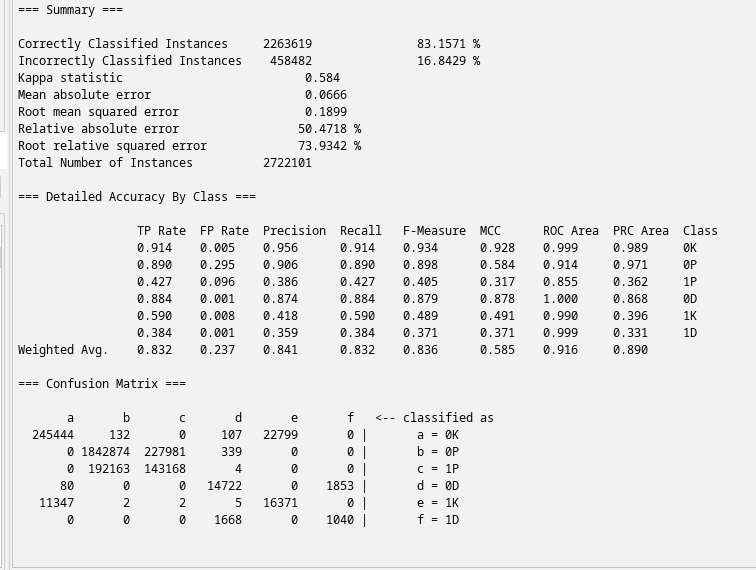
\includegraphics[width=\linewidth]{img/results_bayes.png}
    \caption{Výstup N. Bayes klasifikátoru}
    \label{fig:bayes_results}
\end{figure}
%%%
Dále se ukázalo že z vybraných 13ti atributů, jsou některé téměř irelevantní a proto mohly být z datasetu odstraněny s
minimálním dopadem na výsledky. Tabulka \ref{table:features} reprezentuje vybrané atributy. Odstraněné atributy jsou 
přeškrtnuty. Všechny odstraněné atributy jsou z tabulky \textbf{STUDENTI} a výsledky klasifikace bez těchto atributů
jsou v některých případech i lehce lepší, než s nimi.
\begin{table}[H]
    \begin{center}
        \begin{tabular}{ | c | c | }
            \hline
            Sloupec                       & Alias \\
            \hline \hline
            \sout{NOVE\_PRIJATY}                  & \sout{STD\_NOVE\_PRIJATY}      \\
            \hline
            \sout{STUPEN\_PRED\_VZDELANI}          & \sout{STD\_STUPEN\_PRED\_VZDELANI}      \\
            \hline
            \sout{POCET\_ZAPISOVYCH\_PROPUSTEK}    & \sout{STD\_POCET\_PROPUSTEK}      \\
            \hline
            FORMA                         & SP\_FORMA      \\
            \hline
            FAKULTA\_SP                    & SP\_FAKULTA\_PROGRAMU      \\
            \hline
            \sout{ROK\_PLATNOSTI}                 & \sout{SVR\_ROK}      \\
            \hline
            POC\_KRED                      & ZN\_KREDITY\_ZA\_PREDMET      \\
            \hline
            STATUT                        & ZN\_STATUT\_PREDMETU      \\
            \hline
            POKUS\_CISLO                   & ZN\_POKUS\_CISLO      \\
            \hline
            HODNIDNO\_ZKZP                 & ZN\_HODNOCENI      \\
            \hline
            TYP\_ZK                        & ZN\_TYP\_ZKOUSKY      \\
            \hline
            PRAC\_ZKR                      & ZN\_PRACOVISTE\_ZKRATKA      \\
            \hline
            ZAPOCET\_POKUS                 & ZN\_ZAPOCET\_POKUS      \\
            \hline
        \end{tabular}
        \caption{Použité vlastnosti}
        \label{table:features}
    \end{center}
\end{table}
%%%
%%% Zaver
%%%
\section{Závěr}
Z výsledků porovnání vzniklého modelu ku statistickému podílu je vidět, že model je velmi nepřesný, až skoro 
nepoužitelný. Při inspekci použitých atributů bylo zjištěno, že některé atributy model téměř zhoršovaly. Je možné, že
úspěšnost modelu by dosáhla lepších čísel s větším počtem atributů. Ale také je možné, že zkrátka nelze lépe
předpovídat úspěšnost formy studia se známkami jako hlavní zdroj informací.
%%%
%%%
\end{document}
